\documentclass[11pt]{article}
\setlength\parindent{0pt}
\usepackage{amsmath}
\usepackage{amsfonts}
\usepackage{graphicx}
\newcommand{\reffig}[1]{[Figure \ref{#1}]}
\title{Music Visualization Algorithm}
\author{Zachary Kieda\\{Advisor: Jesse Stiles}}
\date{\today}
\begin{document}
\maketitle\documentclass[11pt]{article}
\setlength\parindent{0pt}
\usepackage{amsmath}
\usepackage{amsfonts}
\usepackage{graphicx}
\newcommand{\reffig}[1]{[Figure \ref{#1}]}
\title{Music Generation}
\author{Zachary Kieda\\{Advisor: Jesse Stiles}}
\date{\today}
\begin{document}
\maketitle
\end{document}


Our music visualization display is a closed form display that is generated with two different parameters. In this report we will give an overview of what the generated output is and the generating function. We will then discuss how the parameters modify the qualitative features of the generated output. In section three we discuss the mathematics behind the visualization that we see, and finally in the fourth section we discuss methods of controlling these two parameters in the context of music generation. 

\begin{section}{Program Output}
The color that we output for each pixel $(x, y)$ we generate a single grayscale color $f(x, y) \in \{k \in \mathbb{N}|0 \le k \le 255\}$. We have example output when zoomed in \reffig{fig:vizsmall}, and output when zoomed out \reffig{fig:vizlarge}. 

\begin{figure}[h]
\centering
\includegraphics[width=.9\textwidth]{viz-small.png}
\caption{Visualization with $\alpha = .01$, $\lambda = 1$}
\label{fig:vizsmall}
\end{figure}

\begin{figure}[h]
\centering
\includegraphics[width=.9\textwidth]{viz-large.png}
\caption{Visualization with $\alpha = .3$, $\lambda = 1$}
\label{fig:vizlarge}
\end{figure}

\begin{subsection}{Generating Function}
Let $(x, y)$ be pixels on the screen such that the origin $(0, 0)$ is at the center. Let $\lambda, \alpha \in \mathbb{R}$. The grayscale pattern formed is 
\[f(x, y) = \alpha (x^2 + y^2)^\lambda \mod 255 \]
Mathematically, this function is uninteresting. If we can view this with infinite precision and $\lambda = 1$, we would merely get a hypergeometric paraboloid that goes back to zero in bands. The spacing of these bands decrease as $x^2$ and $y^2$ increase. Indeed, we see this occur when $\alpha$ is very small \reffig{fig:vizsmall}. However, we get a more interesting result when $\alpha$ gets large. We start to see the function take on a recursive behavior even though the solution is closed form! As $\alpha$ grows, we see a large variation in behavior -- which is interesting coming from a single function.\\


We note that when $\alpha = 255 + \alpha'$,
\begin{align*}
f(x, y) &= (255 + \alpha') (x^2 + y^2)^\lambda &\mod 255 \\
&\equiv 255(x^2 + y^2)^\lambda + \alpha'(x^2+y^2)^\lambda & \mod 255\\
&\equiv \alpha' (x^2 + y^2)^\lambda & \mod 255
\end{align*}
Mathematically, we have shown that the function recurses back to its original function when $\alpha$ goes past 255. This is actually not true for very large $\alpha$ due to floating point errors, which will produce variation for large $\alpha$, but we'll assume that they're roughly equivalent.\\
\end{subsection}
\begin{subsection}{Visualization at various $\alpha$}
We show a variety of figures where $\alpha \approx 11$, $\alpha \approx 50$, $\alpha \approx 150$, and $\alpha = 254.85$. Note that in the last one this is similar to a smaller value of $\alpha$. \\

Note: Zoom in to see the details of the image -- the details change as you zoom in (and for a good reason, which we'll explain in Section 3).
\begin{center}
\includegraphics[width=.9\textwidth]{viz-11.png}\\
Figure 3: Visualization with $\alpha \approx 11$ and $\lambda = 1$
\label{fig:viz11}
\end{center}
\stepcounter{figure}
\begin{figure}[h]
\centering
\includegraphics[width=.9\textwidth]{viz-50.png}
\caption{Visualization with $\alpha \approx 50$ and $\lambda = 1$}
\label{fig:viz50}
\end{figure}
\begin{figure}[h]
\centering
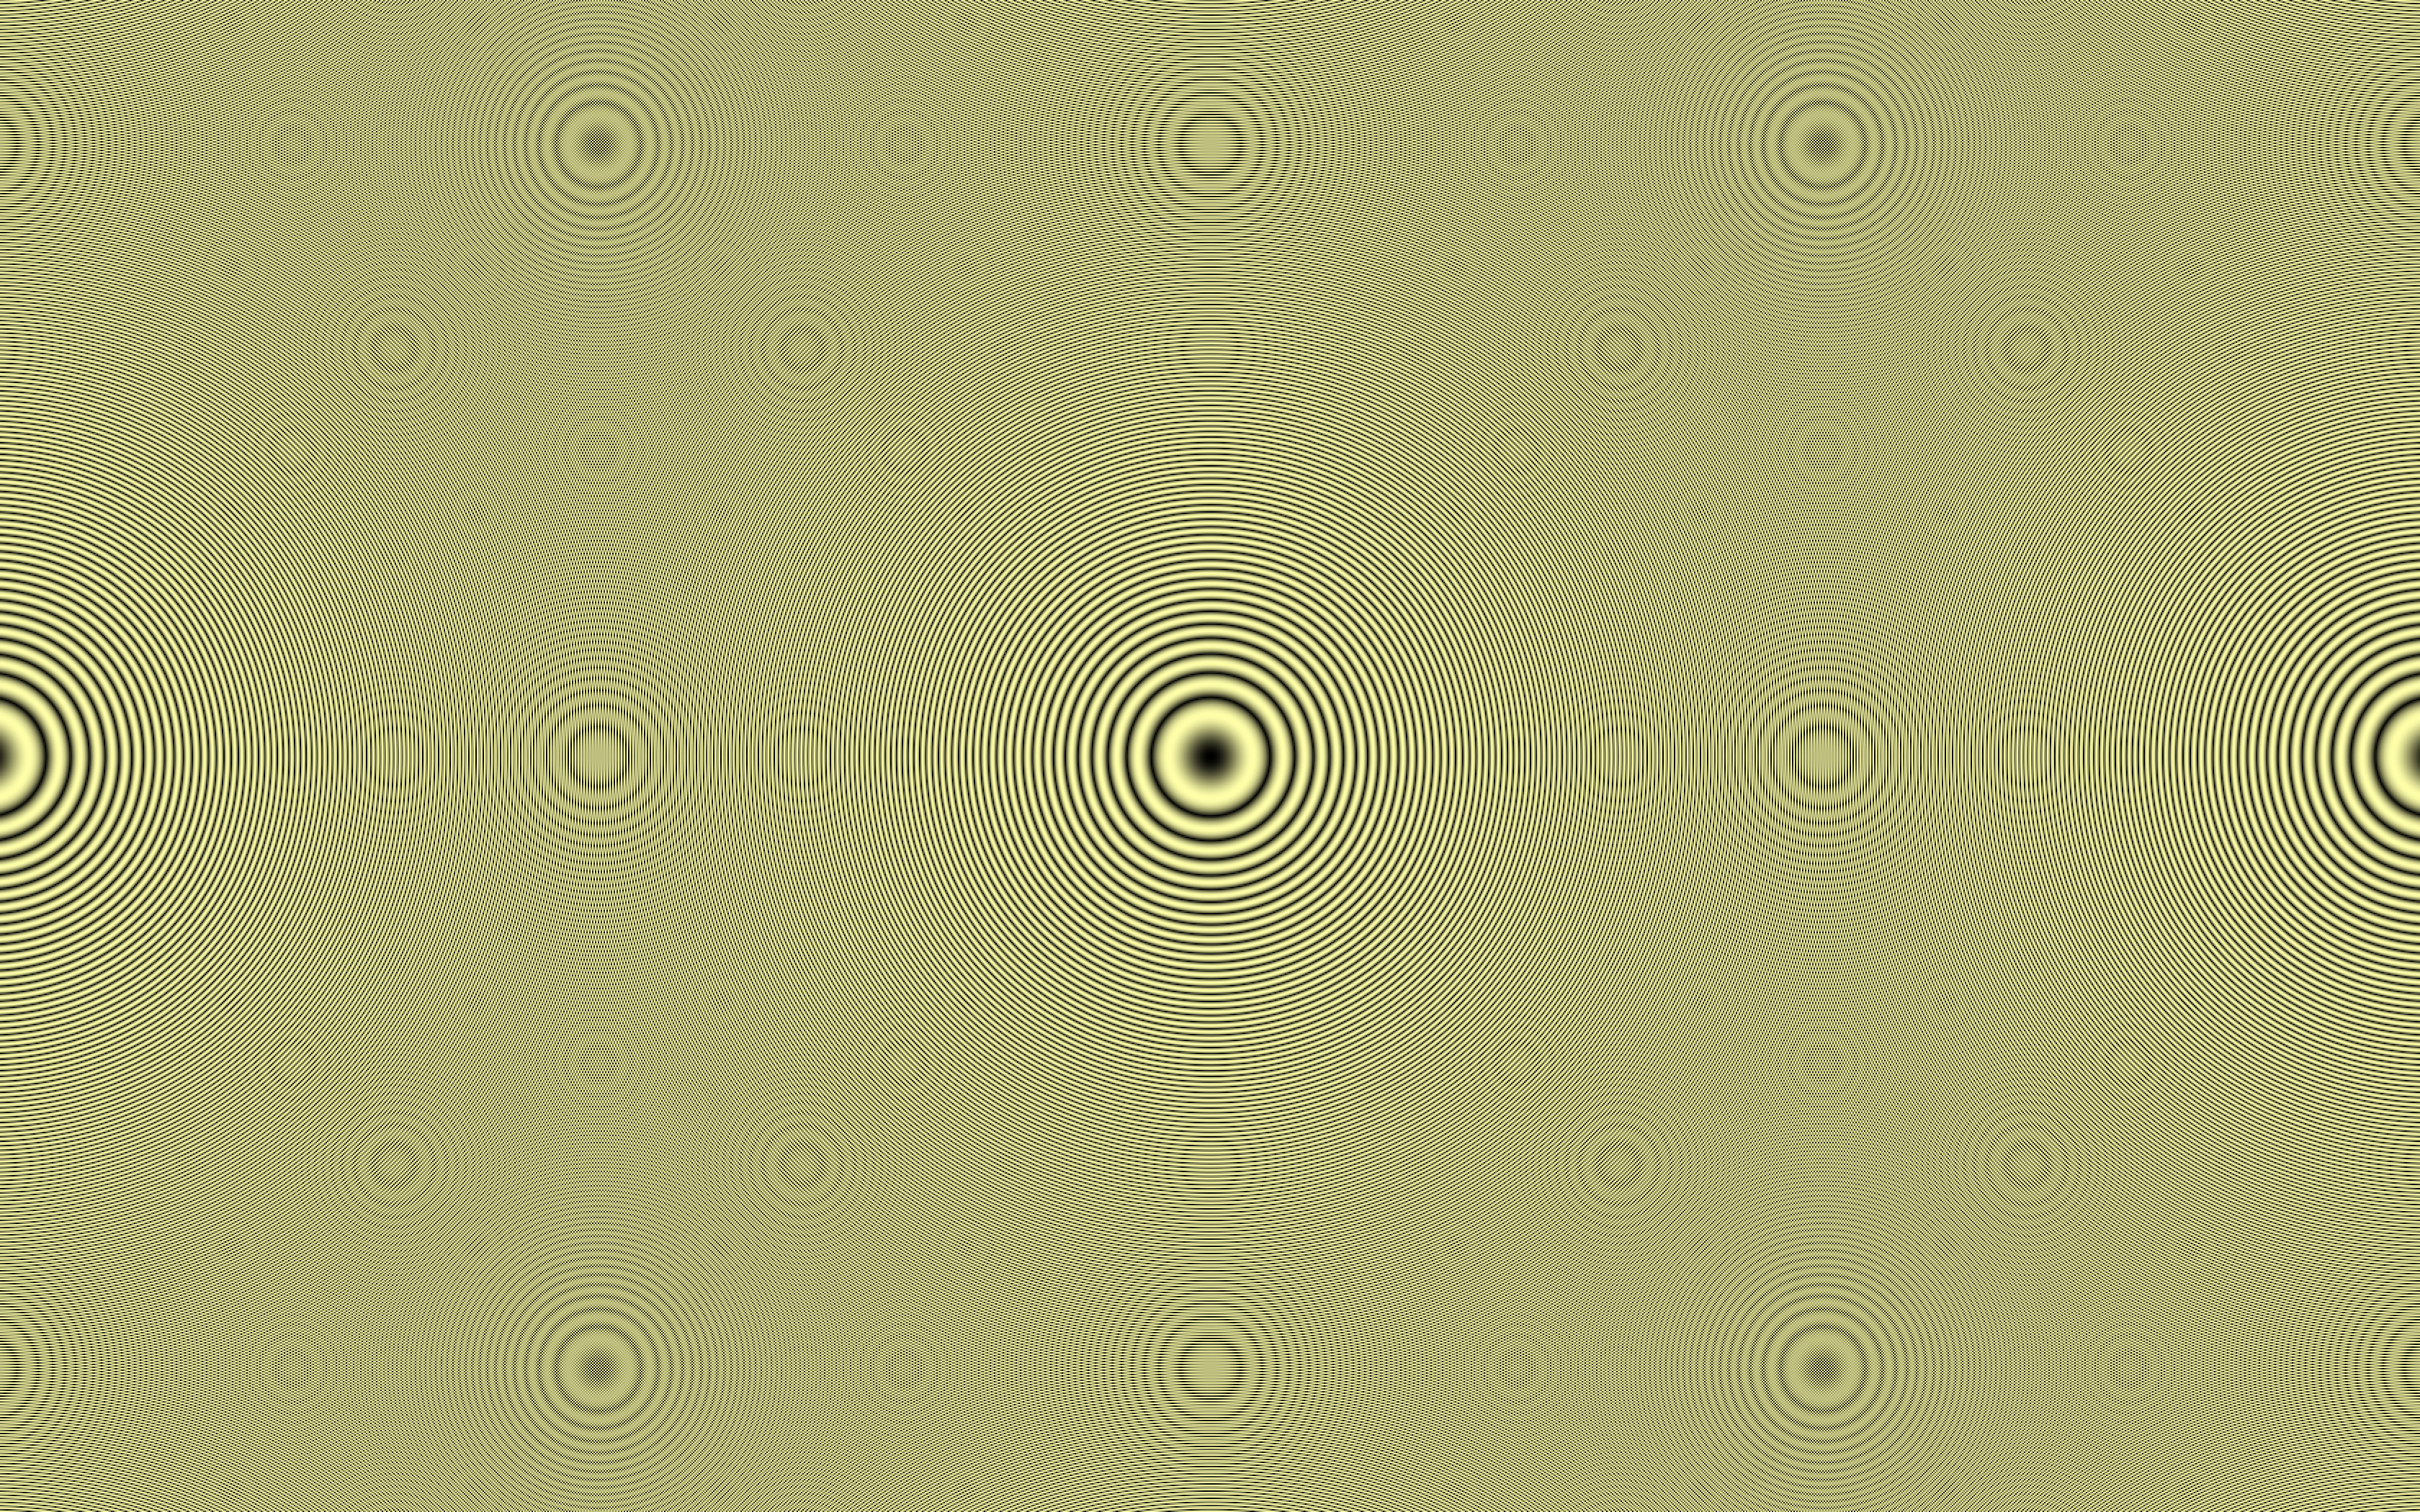
\includegraphics[width=.9\textwidth]{viz-25485.png}
\caption{Visualization with $\alpha = 254.85$ and $\lambda = 1$}
\label{fig:viz25485}
\end{figure}


\end{subsection}
\end{section}
\clearpage
\begin{section}{Additional Qualitative Features and the $\lambda$ Parameter}
\end{section}
\end{document}